\chapter{Evaluación}
\label{chap:evaluation}
\vspace{0.5cm}

%%%%%%%%%%%%%%%%%%%%%%%%%%%%%%%%%%%%%%%%%%%%%%%%%%%%%%%%%%%%%%%%%%%%%%%%%%%%%%%%
% Objetivo: Exponer los resultados objetivos del sistema                       %
%%%%%%%%%%%%%%%%%%%%%%%%%%%%%%%%%%%%%%%%%%%%%%%%%%%%%%%%%%%%%%%%%%%%%%%%%%%%%%%%

 \lettrine{E}{n} este capítulo exponen los resultados de la evaluación del sistema. Se han seleccionado tres piezas musicales conocidas para realizar las diferentes pruebas. A continuación se describen las tres piezas y las pruebas realizadas. Para realizar una prueba de carga que establezca los límites del sistema se ha añadido una última partitura suficientemente sencilla sobre la que trabajar para poder realizar estas pruebas cómodamente sin preocuparse por la calidad de los resultados.
 
 \begin{itemize}
 	\item \textbf{Menuet:} Famosa pieza de Johann S. Bach, destaca por su simpleza y es interesante para ver como funciona el programa ante compases ternarios. Se sugiere añadir una voz nueva de tesitura más aguda a la presente en la pieza.
 	\item \textbf{Greensleves:} Supuestamente compuesta por Enrique VIII, esta archiconocida partitura presenta una polifonía coral a cuatro voces, ideal para comprobar las capacidades de armonización del sistema. Se sugiere eliminar secciones grandes de la voz solista y ver cómo la completa.
 	\item \textbf{Joy to the World:} Conocido villancico, sería interesante escuchar una reinterpretación de la voz más grave para la pieza, ya sea completando secciones o bien añadiendo una voz de bajo.
    \item \textbf{Twinkle Twinkle Little Star:} Esta sencilla pieza tradicional infantil es adecuada para realizar, además de pruebas similares a otras piezas, pruebas de carga para comprobar como crecen los tiempos de búsqueda y hallar los límites de la herramienta.
 \end{itemize}
 
 Para la evaluación se han realizado armonizaciones de todas las piezas y se han medido los tiempos y la calidad de las mismas, además se han realizado pruebas de completado de un compás en cada pieza junto con la inclusión de una nueva voz, también se han medido calidad y tiempo. Por último, con la última partitura se han realizado pruebas para comprobar hasta donde funciona bien en cuestión temporal, para ello se ha ido vaciando porcentualmente una de las voces para ser completada y después se han ido añadiendo diferentes voces. Las figuras de esta sección sirven para ilustrar algunos resultados obtenidos, se puede comparar con las partituras originales presentes en el Apéndice \ref{chap:scores} Partituras.
 
 Nótese que debido al carácter no-determinista de \textit{Answer Set Programming} y a los tiempos de entrada y salida estos tiempos sirven para dar una idea aproximada de los tiempos de funcionamiento de la herramienta. Para suavizar los valores dispares se ha ejecutado cada medida 100 veces, se ha restado el tiempo de usuario y se ha calculado el tiempo promedio. 
 

  \begin{figure}
  	\centering
  	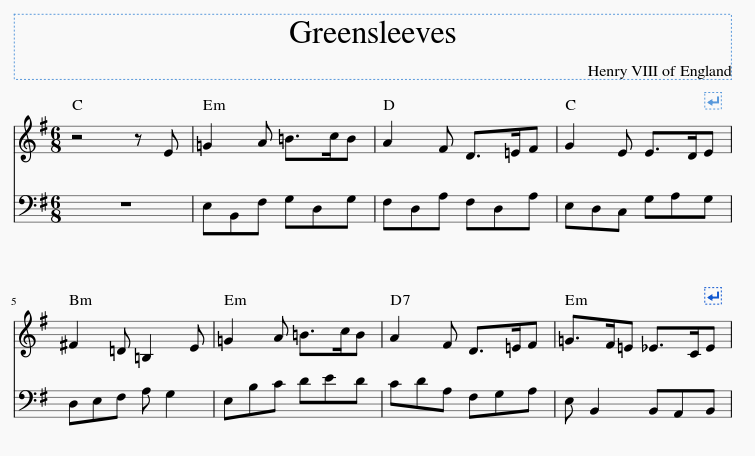
\includegraphics[width=0.8\linewidth]{imagenes/evaluation/greensleeves_harm.png}
  	\caption{Comienzo de Greensleeves armonizado}
  	\label{fig:greensleeves_harm}
  \end{figure}
   
    \begin{figure}
    	\centering
    	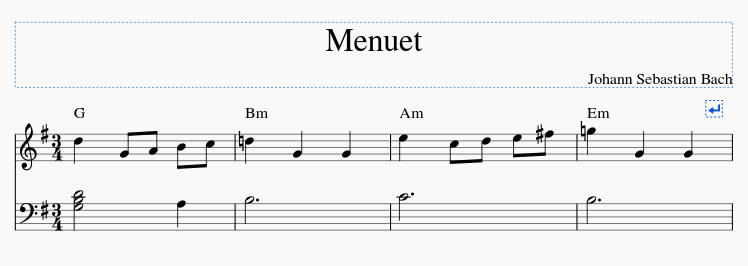
\includegraphics[width=0.8\linewidth]{imagenes/evaluation/menuet_harm.png}
    	\caption{Comienzo de Menuet armonizado}
    	\label{fig:menuet_harm}
    \end{figure}
  
        \begin{figure}
        	\centering
        	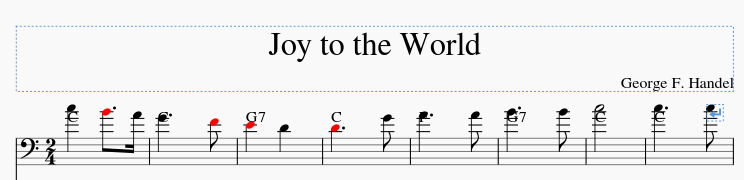
\includegraphics[width=0.8\linewidth]{imagenes/evaluation/joy_harm_err.png}
        	\caption{La salida de Joy to the World produce un error de clave en la voz de la Soprano}
        	\label{fig:joy_harm_err}
        \end{figure}
     
      \begin{figure}
      	\centering
      	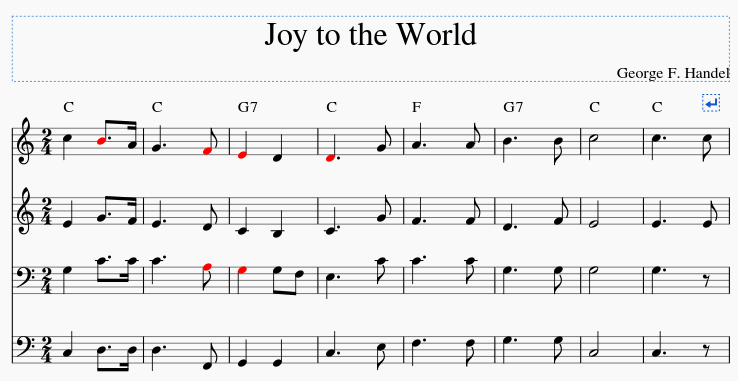
\includegraphics[width=0.8\linewidth]{imagenes/evaluation/joy_harm.png}
      	\caption{Comienzo de Joy to the World armonizado}
      	\label{fig:joy_harm}
      \end{figure}
  
    \begin{figure}
    	\centering
    	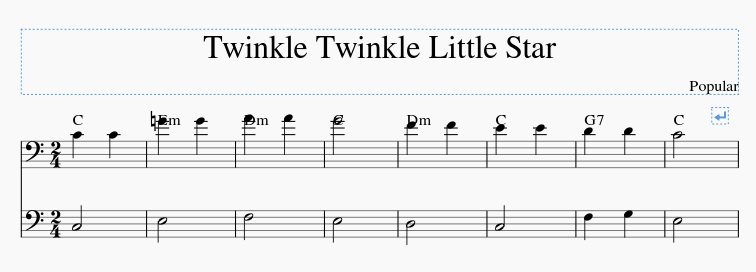
\includegraphics[width=0.8\linewidth]{imagenes/evaluation/twinkle_harm_err.png}
    	\caption{La salida de Twinkle Twinkle Little Star produce un error de clave en la partitura de la mano derecha del piano}
    	\label{fig:twinkle_harm_err}
    \end{figure}
    
        \begin{figure}
        	\centering
        	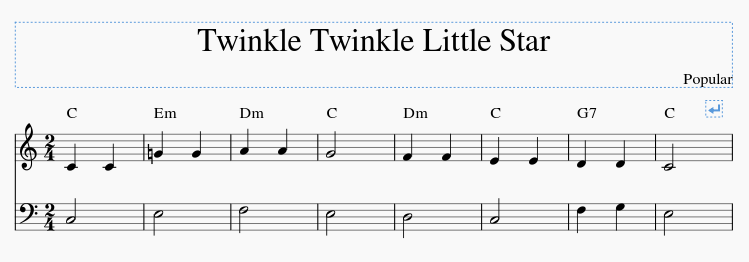
\includegraphics[width=0.8\linewidth]{imagenes/evaluation/twinkle_harm.png}
        	\caption{Comienzo de Twinkle Twinkle Little Star armonizado}
        	\label{fig:twinkle_harm}
        \end{figure}
  
  \begin{center}
  	\begin{tabular}{ | l | c | c | c | }
  		\hline
  		Pieza & T. Armonización & T. Compás & T. Nueva voz \\ \hline \hline
  		Greensleeves &  & 0 & 0 \\ \hline
  		Menuet &  & 0 & 0 \\ \hline
  		Joy to the World &  & 0 & 0 \\ \hline
  		Twinkle Twinkle &  & 0 & 0 \\ \hline
  	\end{tabular}
  \end{center}
  
  \section{Problemas conocidos}
  \label{sec:known_issues}
  Las diferentes pruebas han revelado ciertos problemas que se producen si no siempre, sí lo hacen con una frecuencia relativamente alta y que por diseño de la herramienta no han sido atacados. En la sección de \ref{sec:future_work} Trabajo Futuro en el catulo \ref{chap:conclusiones} Conclusion se detalla cuales de ellos se pretenden arreglar a corto o medio plazo.
  
  \begin{itemize}
  		\item \textbf{Tresillos:} Los tresillos, dosillos y otras figuras irregulares no funcionan correctamente en la herramienta y han de ser editados en la partitura antes de procesarla. Esto se debe a que no es posible realizar una subdivisión directa a la nota base de la partitura de este tipo de figuras.
  		\item \textbf{Clave:} Algunas voces aparecen en la salida con la clave mal identificada, produciendo un resultado poco legible. Esto es fácilmente solucionable cambiando la clave de la voz correspondiente en el archivo de salida, ya que pese a todo, esto es un fallo meramente visual y no afecta a los valores de las notas de la voz.
  		\item \textbf{Nombres de Tesituras:} Si bien los nombres de las voces corales no varían sustancialmente, los nombres de los instrumentos sí lo hacen, por esto el \textit{locale} de la herramienta usada para la edición de partituras puede producir incompatibilidades a la hora de restringir el rango de voces, por ejemplo, una partitura para escrita para Violonchelo en un sistema en castellano marcará esa voz como \texttt{voice\_type(x, violonchelo)} mientras que un sistema en inglés producirá  \texttt{voice\_type(x, violoncello)}. Para solucionarlo se ruega editar el fichero \texttt{voice\_types.lp} en la carpeta \texttt{asp/include} para que los límites de cada instrumento se correspondan con el locale del sistema.
  		\item \textbf{Falsos positivos:} Debido a que en algunas figuras como los conjuntos de corcheas o semicorcheas consecutivas no se puede identificar los subtiempos débiles y fuertes que no dependen del compás si no de la propia figura junto con algunas dificultades a la hora de identificar los tiempos débiles y fuertes de un compás con las notas subdivididas y después transformarlo a otro tipo de compás, es probable que algunas notas marcadas como error en la partitura no lo sean realmente.
  \end{itemize}
  

